\section{Experiments and Results}
\label{sec:experiment}

\subsection{Training Data Preparation}

We first tried to use NBIS \cite{NBIS} to mark the ground truth minutiae and use it for training.
However, we found that the minutiae detection accuracy of NBIS is low.
It will output an image quality number together with the minutiae location and we can set a threshold to select minutiae.
However, the accuracy is low and if we set a high threshold, then many correct minutiae could not be detected, such as the image shown in Fig. \ref{subfig:NBIS-high}.
And if we set a higher threshold, then it will detect many wrong minutiae, as shown in Fig. \ref{subfig:NBIS-low}.
Besides, it cannot find an accurate minutiae threshold, as it either detected a lot of wrong minutiae or miss many important minutiae, or both.
In addition, the locations of much minutiae were wrongly labeled.
For example, in Fig. \ref{subfig:NBIS-low}, three minutiae locations was not correct and we highlight them using yellow color, and we also mark the correct position with red circle.
We can find that there are about 10 pixels gap between the correct minutiae location and those wrongly detected minutiae location, which will make it harder to train a good model.

Therefore, we decide to mark the ground truth minutiae ourselves using labelme \cite{labelme}.
Because it is difficult to find some latent minutiae in the original image, we first enhance the original fingerprint image by estimating the orientation first and then binarizing with the orientations \cite{caoFingerprintImageEnhancement2017}.
After that, we merge the binarized enhanced images with the original images, and then use labelme to manually mark the minutiae on the merged images.
We did not directly use the binarization enhanced images because that there are much wrong minutiae in the enhanced images, therefore we should refer the original images too.
Fig. \ref{subfig:manually-label} presents an example of the the merged images and our manually marked minutiae.
It is the same image as Fig. \ref{subfig:NBIS-low} and \ref{subfig:NBIS-high}, where our manually marked minutiae is much more accurate than them.

\begin{figure}[htbp]
    \centering
    \subcaptionbox{Minutiae detected by NBIS (with a high quality threshold)\label{subfig:NBIS-high}}{
        \includegraphics[width=.3\linewidth]{fig/label/nbis-high-thre.pdf}
    }
    \quad
    \subcaptionbox{Our manually marked minutiae\label{subfig:manually-label}}{
        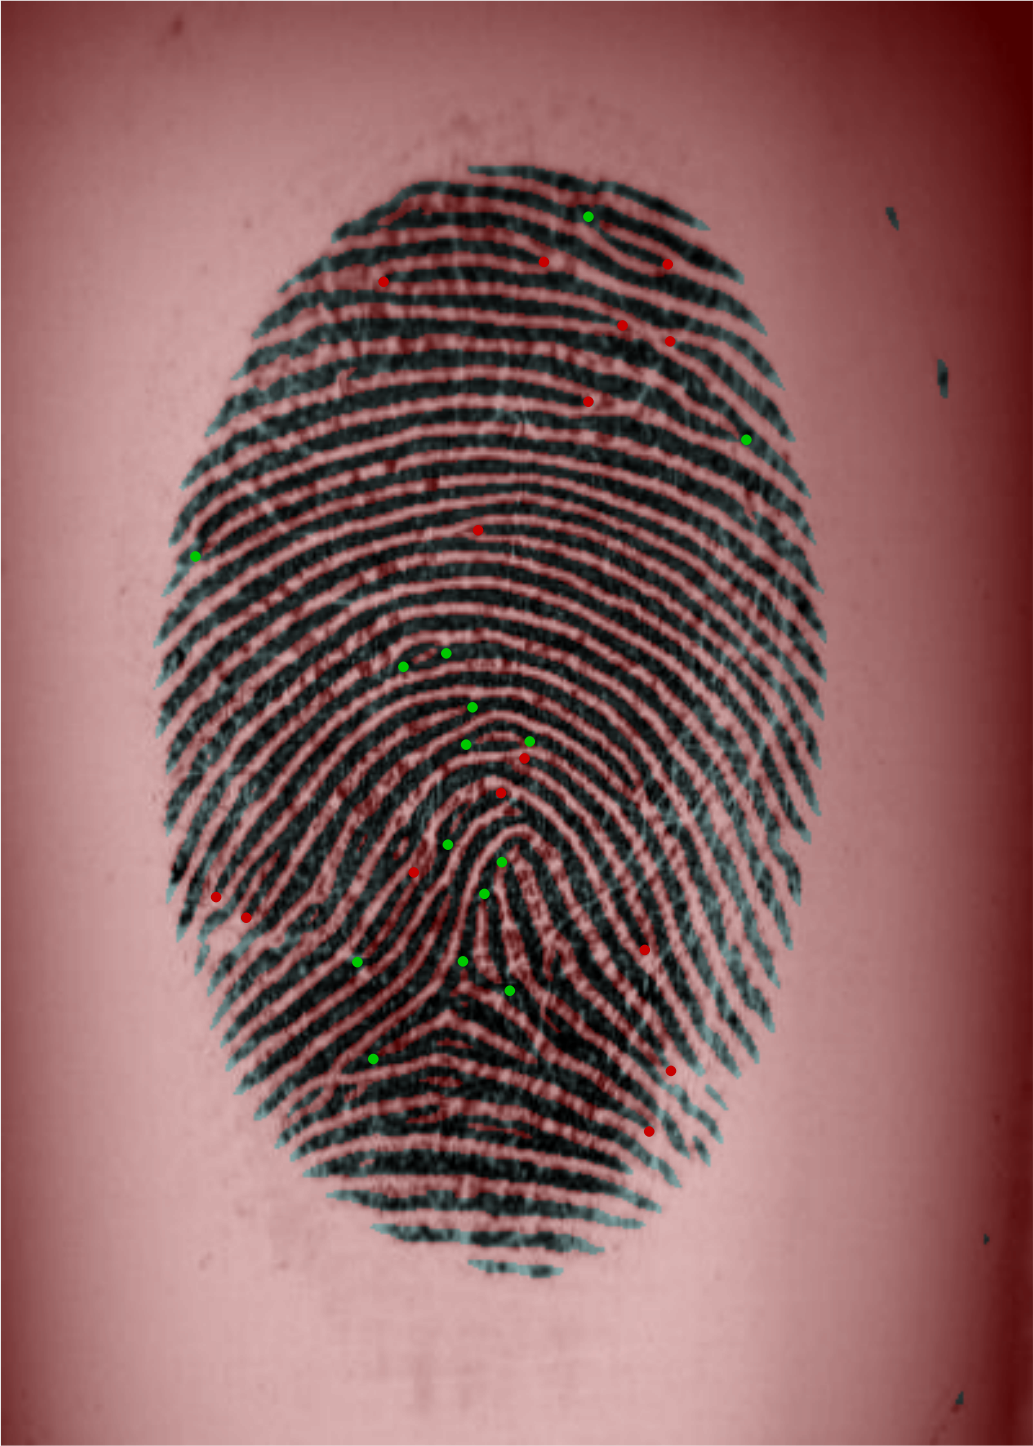
\includegraphics[width=.3\linewidth]{fig/label/manually.png}
    }
    \quad
    \subcaptionbox{Minutiae detected by NBIS (with a low quality threshold)\label{subfig:NBIS-low}}{
        \includegraphics[width=.3\linewidth]{fig/label/nbis-low-thre.pdf}
    }
    \caption{A sample manually marked minutiae with corresponding NBIS detected minutiae}
    \label{fig:label}
\end{figure}


As a result, we first manually selected 200 fingerprint images from the FVC2006 dataset \cite{FVC2006} and marked them manually.
Because we thought these images were not enough and therefore we also manually selected 300 more different high quality fingerprint images which minutiae detection are relatively accurate.
These images are all very clear and the most minutiae was detected by minutiae.
We set a high threshold (35) to filter the incorrect minutiae and get the ground truth minutiae (although there was some missed minutiae and little wrongly detected minutiae).

\def\subwidth{.3}
\begin{figure}[htbp]
    \centering
    \begin{minipage}{.48\linewidth}
        \subcaptionbox{
            original image
        }{
            \includegraphics[width=\subwidth\linewidth]{fig/mask/ori-0.png}
        }
        \subcaptionbox{
            minutiae map
            \label{subfig:not-good-1}
        }{
            \includegraphics[width=\subwidth\linewidth]{fig/mask/mask-0.png}
        }
        \subcaptionbox{
            merged image
        }{
            \includegraphics[width=\subwidth\linewidth]{fig/mask/merge-0.png}
        }
    \end{minipage}
    \quad
    \begin{minipage}{0.48\linewidth}
        \subcaptionbox{
            original image
        }{
            \includegraphics[width=\subwidth\linewidth]{fig/mask/ori-1.png}
        }
        \subcaptionbox{
            minutiae map
        }{
            \includegraphics[width=\subwidth\linewidth]{fig/mask/mask-1.png}
        }
        \subcaptionbox{
            merged image
            \label{subfig:good-1}
        }{
            \includegraphics[width=\subwidth\linewidth]{fig/mask/merge-1.png}
        }
    \end{minipage}
    \newline
    \begin{minipage}{.48\linewidth}
        \subcaptionbox{
            original image
        }{
            \includegraphics[width=\subwidth\linewidth]{fig/mask/ori-2.png}
        }
        \subcaptionbox{
            minutiae map
            }{
            \includegraphics[width=\subwidth\linewidth]{fig/mask/mask-2.png}
        }
        \subcaptionbox{
            merged image
            \label{subfig:good-2}
        }{
            \includegraphics[width=\subwidth\linewidth]{fig/mask/merge-2.png}
        }
    \end{minipage}
    \quad
    \begin{minipage}{0.48\linewidth}
        \subcaptionbox{
            original image
        }{
            \includegraphics[width=\subwidth\linewidth]{fig/mask/ori-3.png}
        }
        \subcaptionbox{
            minutiae map
        }{
            \includegraphics[width=\subwidth\linewidth]{fig/mask/mask-3.png}
        }
        \subcaptionbox{
            merged image
            \label{subfig:not-good-2}
        }{
            \includegraphics[width=\subwidth\linewidth]{fig/mask/merge-3.png}
        }
    \end{minipage}

    \caption{Some sample images and predicted minutiae map}
    \label{fig:minutiae-map}
\end{figure}


\subsection{Minutiae Detection}

We test our model using the rest of the fingerprint images in FVC2006 dataset.
Fig \ref{fig:minutiae-map} presents some randomly selected sample images and corresponding minutiae map.
We also merge the original images and the predicted minutiae map to make it more clear to view.
From Fig. \ref{fig:minutiae-map}, we can find that the minutiae in sub-figure \ref{subfig:good-1} and \ref{subfig:good-2} are very accurate.
Almost every minutiae is detected and there is not wrongly detected minutiae.
The minutiae in \ref{subfig:not-good-1} and \ref{subfig:not-good-2} is a little worse, where a few minutiae in the noisy area is wrongly detected.

The minutiae detection results are much better than existing algorithms, such as MinutiaeNet \cite{NguyenICB2018}.
We used the source code provided in \cite{NguyenICB2018} and calculate the corresponding minutiae.
Fig. \ref{fig:minutiaenet-results} presents some sample minutiae detection results.
We can easily find that there is a lot of wrongly detected minutiae and missed minutiae.
Due to the time limitation, we did not implement other deep learning based algorithms and make comparison, but based on the detection results, we think our minutiae detection network achieve a very high accuracy and may surpass many existing minutiae detection algorithms.
% , therefore we refer the minutiae detection results in the papers and make a simple comparison.

\def \figwidth {.19}
\begin{figure}[htbp]
    \centering
    \includegraphics[width=\figwidth\linewidth]{fig/minutiaenet/1.jpg}
    \includegraphics[width=\figwidth\linewidth]{fig/minutiaenet/2.jpg}
    \includegraphics[width=\figwidth\linewidth]{fig/minutiaenet/3.jpg}
    \includegraphics[width=\figwidth\linewidth]{fig/minutiaenet/4.jpg}
    \includegraphics[width=\figwidth\linewidth]{fig/minutiaenet/5.jpg}
    \caption{Some sample minutiae detection results of MinutiaeNet \cite{NguyenICB2018}}
    \label{fig:minutiaenet-results}
\end{figure}

% After detect the minutiae, we then use non maximum suppression to locate the minutiae.




\subsection{Graph Triplet}

We use MNIST dataset \cite{LecunIEEE1998} to build the graph triplet, and use SplineCNN layer \cite{FeyCVPR2018splinecnn} \cite{FeyICLR2020DGMC} to replace the CNN layer which is normally used in computer vision task. Each MNIST image is represented as a graph, whose nodes correspond to the pixels in the image and the edge is formed by connected each pixel to all its neighboring pixels. Therefore, based on this setup, each MNIST image is a graph with the same number of nodes, which is $784(=28^2)$. The graph triplet is formulated as follows: for each sample as the anchor in the training dataset, we randomly select another sample which belongs to the same class as the positive sample, and randomly select one sample from the rest classes as the negative sample. 

Similar to CNN neural network configuration, we build a SplineCNN network, which contains two SplineCNN layers, and ech SplineCNN layer is followed by an exponential linear unit (ELU) and a max-pooling layer. There are two fully connected layers, the first fully connected layer is also followed by an ELU layer, the output dimension of the final fully connected layer is $10$ (we also choose the final dimension to be $2$ for visualization). The initial learning rate is $10^{-3}$. Stochastic gradient descent with Adam method is used for optimization and the total training epochs is $20$.

\begin{figure}[htb]
    \begin{minipage}[b]{0.48\linewidth}
        \centering
        \centerline{\epsfig{figure=./image/mnist_plot/train_plot.png, height=7.0cm}}
        % \caption{MNIST training set result}
        % \label{fig:mnist_train_plot}
    \end{minipage}
    \hfill
    \begin{minipage}[b]{0.48\linewidth}
        \centering
        \centerline{\epsfig{figure=./image/mnist_plot/test_plot.png, height=7.0cm}}
        % \caption{MNIST test set result}
        % \label{fig:mnist_test_plot}
    \end{minipage}
    \caption{Visualization of MNIST training set and test set result}
    \label{fig:mnist_plot}
\end{figure}

For evaluation, since the total number of samples of MNIST test dataset is $10,000$ and they are not balanced for each class, we randomly choose 500 samples from each class. We use all-to-all evaluation protocol, which means for each test sample, Euclidean distance is computed against all the rest samples. Therefore, in total, we generate $1,247,500$ genuine scores and $11,250,000$ impostor scores. Since MNIST dataset is a simple dataset with a few number of classes and a large number of samples for each class, it turns out that there is no overlap between genuine scores and impostor scores. The equal error rate(EER) is thus zero.

